\chapter{Interfacing a Potentiometer}
\thispagestyle{empty}
\label{potmeter}

\newcommand{\LocPotfig}{\Origin/user-code/pot/figures}
\newcommand{\LocPotscicode}{\Origin/user-code/pot/scilab}
\newcommand{\LocPotscibrief}[1]{{\tt
    \seqsplit{Origin/user-code/pot/scilab/#1}}, 
see \fnrefp{fn:file-loc}}
\newcommand{\LocPotardcode}{\Origin/user-code/pot/arduino}
\newcommand{\LocPotardbrief}[1]{{\tt
    \seqsplit{Origin/user-code/pot/arduino/#1}},
see \fnrefp{fn:file-loc}}

%%%%%%%%%%%%%%%python starts
\newcommand{\LocPotpycode}{\Origin/user-code/pot/python}
\newcommand{\LocPotpybrief}[1]{{\tt
    \seqsplit{Origin/user-code/pot/python/#1}},
see \fnrefp{fn:file-loc}}
%%%%%%%%%%%%%%%python ends

%%%%%%%%%%%%%%%julia starts
\newcommand{\LocPotjuliacode}{\Origin/user-code/pot/julia}
\newcommand{\LocPotjuliabrief}[1]{{\tt
    \seqsplit{Origin/user-code/pot/julia/#1}},
see \fnrefp{fn:file-loc}}
%%%%%%%%%%%%%%%julia ends

%%%%%%OpenModelica starts
\newcommand{\LocPotOpenModelicacode}{\Origin/user-code/pot/OpenModelica}
\newcommand{\LocPotOpenModelicabrief}[1]{{\tt
    \seqsplit{Origin/user-code/pot/OpenModelica/#1}},
see \fnrefp{fn:file-loc}}
%%%%%%OpenModelica ends

A potentiometer is a three-terminal variable resistor with two
terminals connected to the two ends of a resistor and one connected to
a sliding or rotating contact, termed as a wiper. The wiper can be
moved to vary the resistance, and hence the potential, between the
wiper and each terminal of the resistor. Thus, a potentiometer
functions as a variable potential divider. It finds wide application
in volume control, calibration and tuning circuits, motion control,
joysticks, etc.

In this chapter, we will perform an experiment to read the analog
values from a potentiometer mounted on the shield of \arduino\
board. The analog values read from the potentiometer will then be
used to control the actuation of other components.

\section{Preliminaries}
The shield provided with the kit has a 1K potentiometer mounted on
it. The mechanical contact at the middle terminal is rotated to vary
the resistance across the middle terminal and the two ends of the
potentiometer. With the fixed voltage across the two terminals of the
potentiometer, the position of the wiper determines the potential
across the middle terminal and either of the two end
terminals. Nowadays, digital potentiometer integrated circuits, which
vary resistance across two pins on the basis of the set value, are
also available.

\begin{figure}
\centering
\subfloat[Pictorial representation of a potentiometer]{
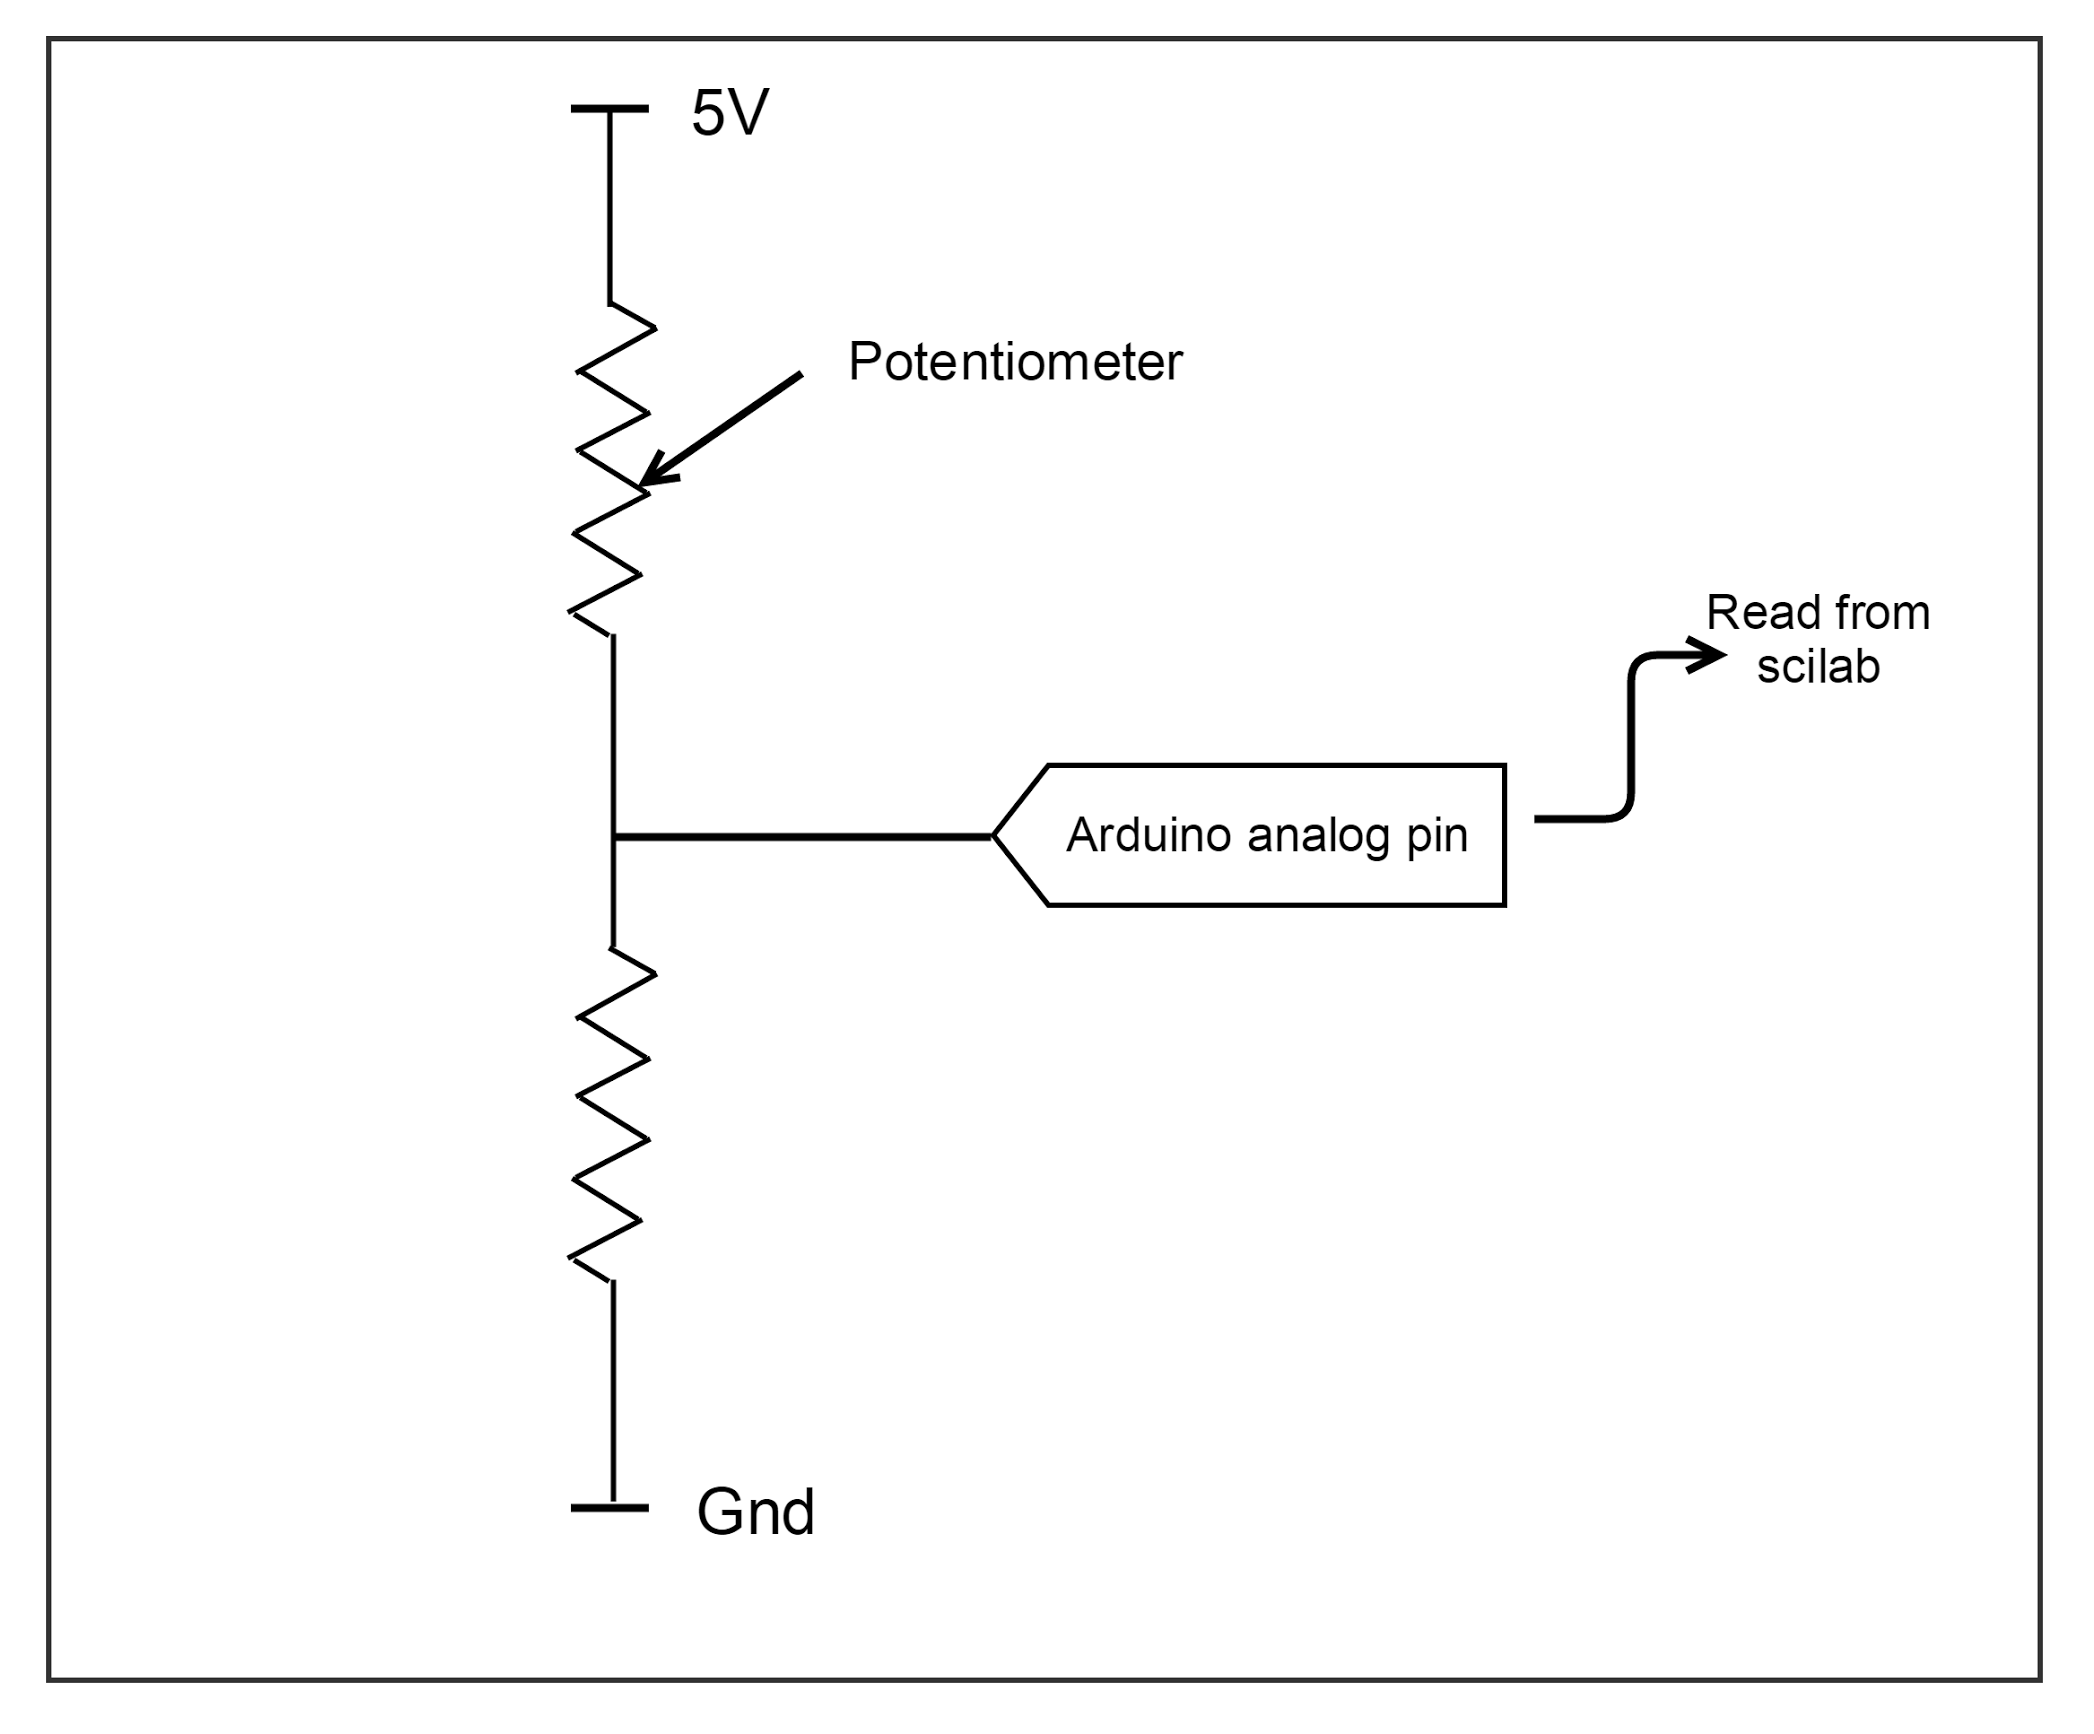
\includegraphics[width=\smfig]{\LocPotfig/potmeter.png}
\label{fig:pot}} \hfill
\subfloat[Internal connection diagram for the potentiometer on the shield]{
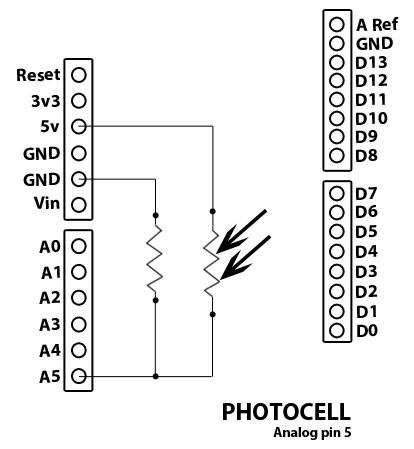
\includegraphics[width=\smfig]{\LocPotfig/schematic.png}
\label{fig:potsch}}
\caption{Potentiometer's schematic on the shield}
\label{fig:potmeterconn}
\end{figure}

The potentiometer used in the kit can be seen on the shield in
\figrefp{fig:uno-shield-connect}.  It is
mounted on the shield. The two end terminals of the potentiometer are
connected to 5V supply and ground. The middle terminal is connected to
analog pin 2 of the \arduino\ board. The resistance between the middle
terminal and either of the two ends can be varied by rotating the
middle terminal by hand. The connection diagram for the potentiometer
is shown in \figref{fig:potmeterconn}.

The reading of a potentiometer is an analog voltage varying from 0 to
5V. Like LDR, we use the ADC functionality of the
\arduino\ board. Thus, we obtain digital values between 0 and 1023. 
% Scilab Console or Arduino Serial Monitor.
% redcolor{Arduino Serial Monitor}
In the experiment explained in this chapter, we shall also use an RGB
LED mounted on the shield. An RGB LED is a tri-color LED which can
illuminate in Red, Green, and Blue colors. It has 4 leads of which one
lead is connected to ground and other three leads are connected to
digital I/O pins 9, 10, and 11 of Arduino. In order to switch on a
particular LED, we need to provide HIGH (5V) voltage to the
corresponding pin of the \arduino\ board.

\section{Connecting a potentiometer with \arduino\ using a breadboard}
This section is useful for those who either don't have a shield or don't want to use the shield
for performing the experiments given in this chapter. 

A breadboard is a device for holding the components of a circuit and connecting 
them together. We can build an electronic circuit on a breadboard without doing any 
soldering. To know more about the breadboard and other electronic components, 
one should watch the Spoken Tutorials on Arduino as published on
{\tt https://spoken-tutorial.org/}. Ideally, one should go through all the
tutorials labeled as Basic. However, we strongly recommend the readers should
watch the fifth and sixth tutorials, i.e., {\tt First Arduino Program} and 
{\tt Arduino with Tricolor LED and Push button}.

In case you have a potentiometer, and you want to connect it with \arduino\ on a breadboard, 
please refer to \figref{fig:pot-led}. The connections given in this figure 
can be used to control an RGB LED depending upon the values from the potentiometer.  
\begin{figure}
  \centering
  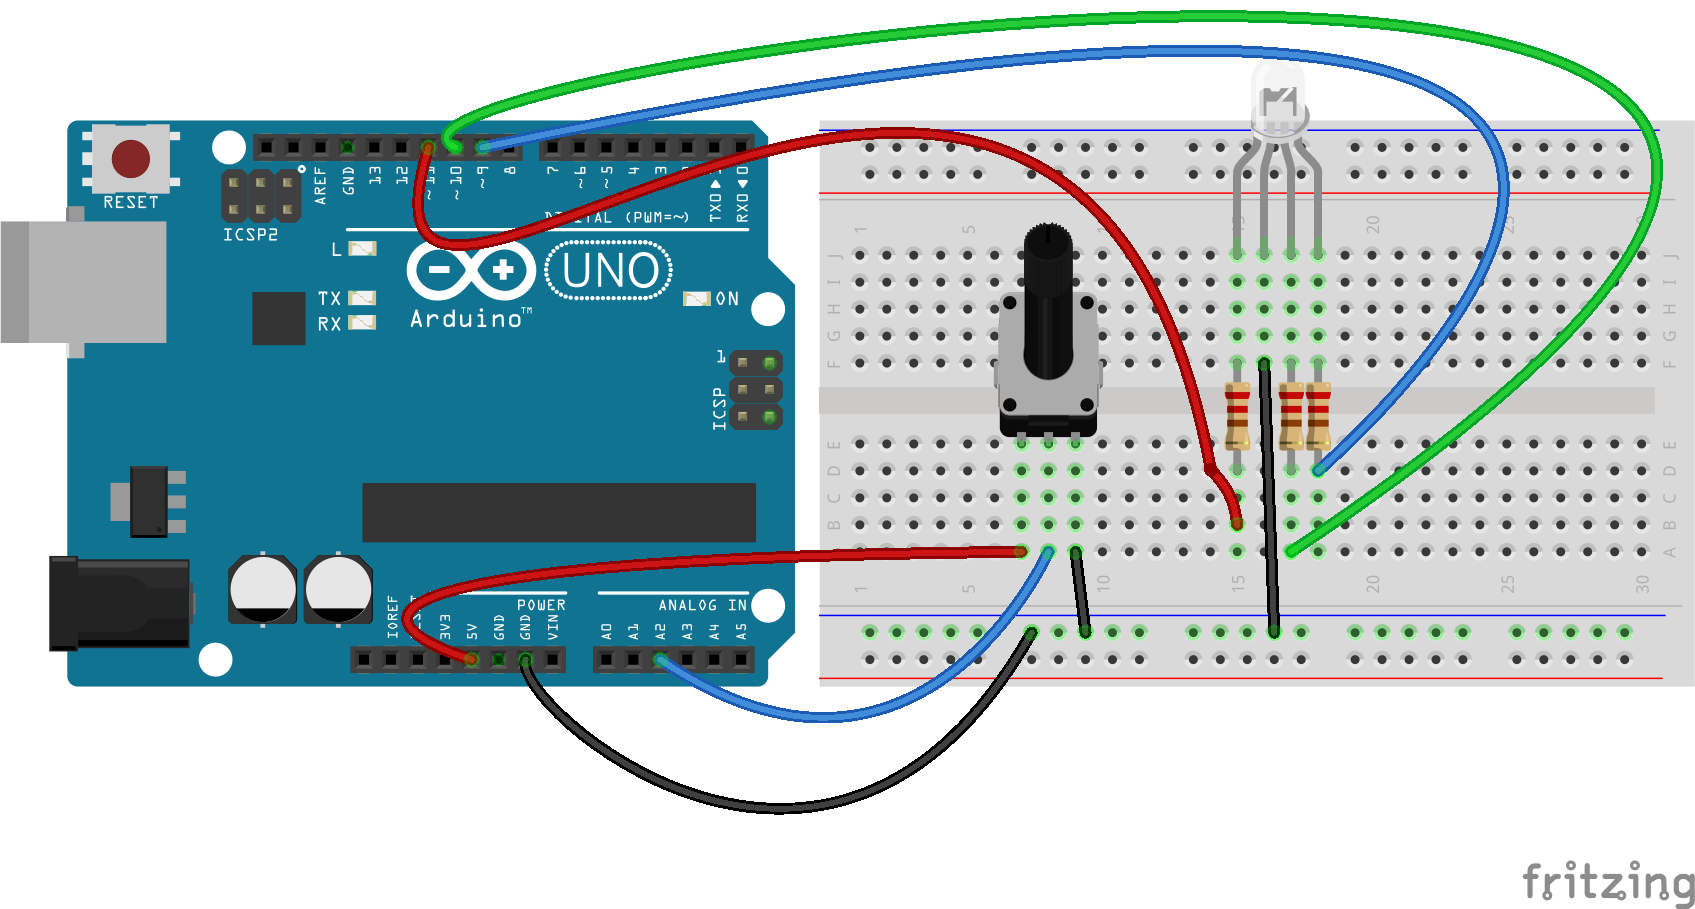
\includegraphics[width=\textwidth]{\LocPotfig/POT-led-bb.png}
  \caption{A potentiometer to control an LED with Arduino Uno using a breadboard}
  %\redcolor{connected on pin no. D12}}
  \label{fig:pot-led}
\end{figure}
As shown in \figref{fig:pot-led}, the three legs of the potentiometer are connected to 
5V, analog pin 2, and GND on \arduino. Depending upon how much the potentiometer's shaft is rotated, one can get a value on analog pin 2. On the other hand, 
there is an RGB LED, and its four legs are connected to three different digital pins and GND on \arduino\, as discussed in 
\chapref{led}. 


\section{Reading the potentiometer from the Arduino IDE}
\subsection{Reading the potentiometer}
In this section, we shall learn how to read the potentiometer 
input through Arduino IDE. Depending on the acquired potentiometer 
values, we will change the state of the RGB LED. The shield has to be attached to the \arduino\ board
before doing this experiment and the \arduino\ needs to be connected to the computer 
with a USB cable, as shown in \figref{arduino}. The reader should go through the
instructions given in \secref{sec:ard-start} before getting started.

The Arduino code for this experiment is given in \ardref{ard:pot-100}. 
In this code, lines 1 through 4 are used to assign relevant PINs to 
the potentiometer and RGB LED. The purpose of these lines is to avoid 
confusion, with the PINs, for beginners. Next, we start serial port 
communication, as on line 9, with the baud rate of 115200. 
To take the potentiometer input, we need to initialize the pins by 
giving the following commands:

\lstinputlisting[firstline=9,lastline=12]
{\LocPotardcode/pot-threshold/pot-threshold.ino}

where {\tt pinMode} command is used to configure the specified pin as
an input or an output pin. The first argument for the above command
corresponds to the pin number and second argument corresponds to the
mode of operation. In this experiment, we configure digital pin 2 as
an input pin while digital pins 9, 10, and 11 as output pins. Next, we
check the value of potentiometer using {\tt analogRead} command for 10
iterations. These values range from 0 to 1023. Depending on the read
value, we turn on and turn off the Red, Green or Blue LED. For
example, when the position of the potentiometer corresponds to the
values between 0 and 319, inclusive, we turn on the Red LED, keep it
on for 1000 ms and then turn it off. This functionality is carried out
by,
\lstinputlisting[firstline=16,lastline=19]
                {\LocPotardcode/pot-threshold/pot-threshold.ino}
In a similar manner,
we check the potentiometer values and correspondingly turn on and off
the Green and Blue LEDs. Note that, we have used {\tt if and else if}
statements to check the conditions. While running this experiment, 
the readers must rotate the knob of the potentiometer and observe 
the change in the color of the RGB LED.  

\subsection{Arduino Code}
\lstset{style=mystyle}
\label{sec:pot-arduino-code}
\addtocontents{ard}{\protect\addvspace{\codclr}}

\begin{ardcode}
  \acaption{Turning on LEDs depending on the potentiometer
    threshold}{Turning on LEDs depending on the potentiometer
    threshold.  Available at
    \LocPotardbrief{pot-threshold/pot-threshold.ino}.}
\label{ard:pot-100}
\lstinputlisting{\LocPotardcode/pot-threshold/pot-threshold.ino}
\end{ardcode}

